%!TEX root = ../thesis.tex

\section{Appendix: Unused theorems}


\begin{thrm}
\label{th:irreducible and chordfree triangulation of the kgon is 3connected}
A irreducible triangulation $G$ of the $k$-gon with a chordfree outer cycle is $3$-connected.
\end{thrm}
\begin{proof}
  This proof has to be expanded.

  The completion $G'$ is a irreducible triangulation. Chordfree outer cycle is important, because a chord will form a separating triangle in $G'$.
\end{proof}

\begin{thrm}
  Any irreducible triangulation $T$ of the $4$-gon with $n \geq 5$ is $3$-connected.
\end{thrm}
\begin{proof}
  Let us name the four vertices of the outer cycle $a,b,c,d$, this cycle has at least one interior vertex $v$ since $n\geq 5$. The edges $ac$ and $bd$ can not exist since they would create a separating triangle containing $v$. hence the outer cycle is chordfree.
  Theorem \ref{th:irreducible and chordfree triangulation of the kgon is 3connected} then concludes the proof
\end{proof}


\begin{thrm}
  Every interior vertex of a triangulation of the $n$-gon has degree at least $3$.
\end{thrm}

\begin{proof}
  This follows directly from Theorem \ref{th:triOfK3:VertexDisjointPaths}. If a interior vertex would have a lower degree it can never have $3$ vertex disjoint paths to the outer cycle.
\end{proof}

%\begin{proof}
%Suppose a interior vertex $v$ has degree $1$ then clearly the face surrounding $v$ can not have degree $3$. Now suppose that an interior vertex $v$ has degree $2$. We then let $u$ and $w$ denote its neighbours and $F$ and $F'$ the face incident to $v$. See also Figure \ref{fig:interiorVertexDegree3}. Then since $F$ and $F'$ are both interior faces they need to be off degree $3$ this implies that $uw$ is an edge for both faces. This is impossible and hence every interior vertex has at least degree $3$
%\end{proof}

%\begin{figure}[h!]
%\centering
%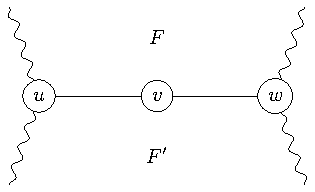
\includegraphics{prelim/img/interiorVertexDegree3.pdf}
%\caption{The notation as described in the proof \label{fig:interiorVertexDegree3}
%}
%\end{figure}
